\chapter{Psalm 41}

\begin{figure}
  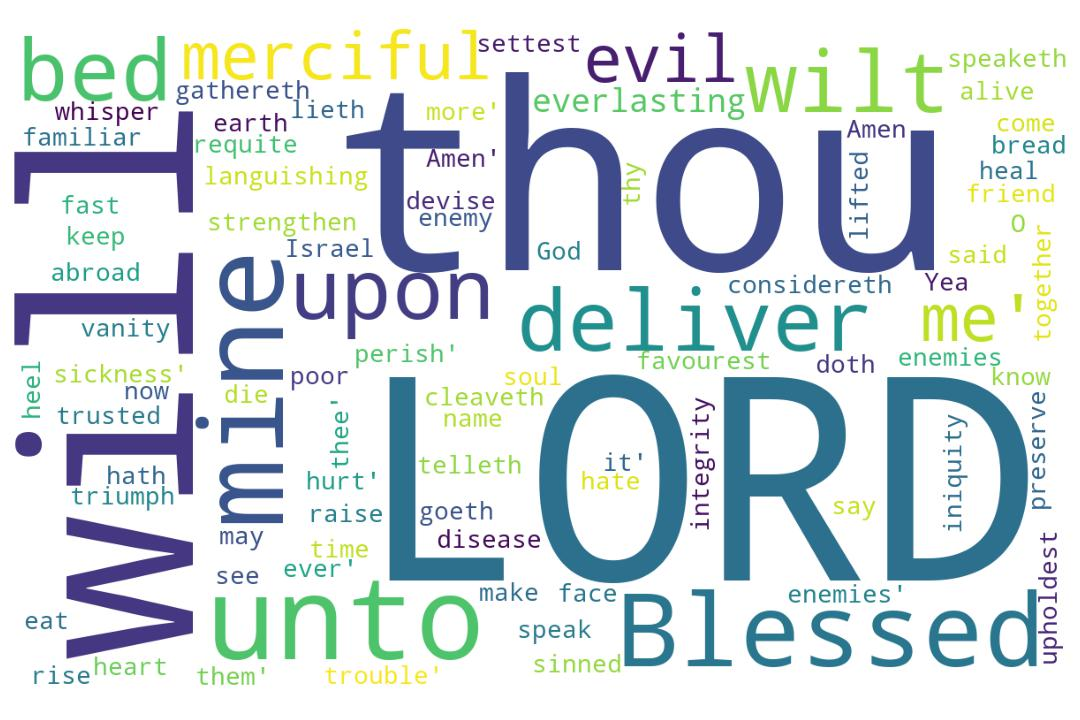
\includegraphics[width=\linewidth]{19OT-Psalms/Psalm41-WordCloud.jpg}
  \caption{Psalm 41 Word Cloud}
  \label{fig:Psalm 41 word Cloud}
\end{figure}

\marginpar{\scriptsize \centering \fcolorbox{bone}{lime}{\textbf{PURE RELIGION}}\\ (Psalm 41:1-13)

\begin{compactenum}[I.][8]
    \item \textbf{Empowers} \index[scripture]{Psalms!Psa 041:01} (Psa  41:1)
    \item \textbf{Preserves} \index[scripture]{Psalms!Psa 041:02} (Psa  41:2)
    \item \textbf{Protects} \index[scripture]{Psalms!Psa 041:02} (Psa  41:2)
    \item \textbf{Prioritizes} (both for you and for God) \index[scripture]{Psalms!Psa 041:11} (Psa  41:11)
    \item \textbf{Perseveres} \index[scripture]{Psalms!Psa 041:13} (Psa 41:13)
    \item \textbf{Pictures} God's Care for the Helpless (like helpless sinners) %\index[scripture]{Psalms!Psa 041:01} (Psalm  41:1)
\end{compactenum}}

\footnote{\textcolor[cmyk]{0.99998,1,0,0}{\hyperlink{TOC}{Return to end of Table of Contents.}}}\footnote{\href{https://audiobible.com/bible/}{\textcolor[cmyk]{0.99998,1,0,0}{Psalms Audio}}}\textcolor[cmyk]{0.99998,1,0,0}{To the chief Musician, A Psalm of David.}\\
\\
\textcolor[cmyk]{0.99998,1,0,0}{Blessed \emph{is} he that considereth the poor: the LORD will \fcolorbox{bone}{lime}{deliver} him in time of trouble.}\footnote{\textbf{Proverb 29:7} - The righteous considereth the cause of the poor: but the wicked regardeth not to know it.}
[2] \textcolor[cmyk]{0.99998,1,0,0}{The LORD will \fcolorbox{bone}{lime}{preserve} him, and keep him alive; \emph{and} he shall be blessed upon the earth: and thou wilt not deliver him unto the \fcolorbox{bone}{lime}{will of his enemies}.}\footnote{\textbf{Genesis 45:4-7} -  And Joseph said unto his brethren, Come near to me, I pray you. And they came near. And he said, I am Joseph your brother, whom ye sold into Egypt. [5] Now therefore be not grieved, nor angry with yourselves, that ye sold me hither: for God did send me before you to preserve life. [6] For these two years hath the famine been in the land: and yet there are five years, in the which there shall neither be earing nor harvest. [7] And God sent me before you to preserve you a posterity in the earth, and to save your lives by a great deliverance.}\footnote{\textbf{Psalm 121} - I will lift up mine eyes unto the hills, from whence cometh my help. [2] My help cometh from the LORD, which made heaven and earth. [3] He will not suffer thy foot to be moved: he that keepeth thee will not slumber. [4] Behold, he that keepeth Israel shall neither slumber nor sleep. [5] The LORD is thy keeper: the LORD is thy shade upon thy right hand. [6] The sun shall not smite thee by day, nor the moon by night. [7] The LORD shall preserve thee from all evil: he shall preserve thy soul. [8] The LORD shall preserve thy going out and thy coming in from this time forth, and even for evermore.}\footnote{\textbf{2 Timothy 4:18} - And the Lord shall deliver me from every evil work, and will preserve me unto his heavenly kingdom: to whom be glory for ever and ever. Amen.}
[3] \textcolor[cmyk]{0.99998,1,0,0}{The LORD will strengthen him upon the bed of languishing: thou wilt make all his bed in his sickness.}
[4] \textcolor[cmyk]{0.99998,1,0,0}{I said, LORD, be merciful unto me: heal my soul; for I have sinned against thee.}
[5] \textcolor[cmyk]{0.99998,1,0,0}{Mine enemies speak evil of \fcolorbox{bone}{bone}{me}, When shall he die, and his name perish?}
[6] \textcolor[cmyk]{0.99998,1,0,0}{And if he come to see \emph{\fcolorbox{bone}{bone}{me}}, he speaketh vanity: his heart gathereth iniquity to itself; \emph{when} he goeth abroad, he telleth \emph{it}.}
[7] \textcolor[cmyk]{0.99998,1,0,0}{All that hate \fcolorbox{bone}{bone}{me} whisper together against \fcolorbox{bone}{bone}{me}: against \fcolorbox{bone}{bone}{me} do they devise my hurt.}
[8] \textcolor[cmyk]{0.99998,1,0,0}{An evil disease, \emph{say} \emph{they}, cleaveth fast unto him: and \emph{now} that he lieth he shall rise up no more.}\footnote{\textbf{Ecclesiates 6:2} - A man to whom God hath given riches, wealth, and honour, so that he wanteth nothing for his soul of all that he desireth, yet God giveth him not power to eat thereof, but a stranger eateth it: this is vanity, and it is an evil disease.}
[9] \textcolor[cmyk]{0.99998,1,0,0}{Yea, mine own familiar friend, in whom I trusted, which did eat of my bread, hath lifted up \emph{his} heel against \fcolorbox{bone}{bone}{me}.}
[10] \textcolor[cmyk]{0.99998,1,0,0}{But thou, O LORD, be merciful unto \fcolorbox{bone}{bone}{me}, and raise \fcolorbox{bone}{bone}{me} up, that I may requite them.}
[11] \textcolor[cmyk]{0.99998,1,0,0}{By this I know that thou \fcolorbox{bone}{lime}{favourest} \fcolorbox{bone}{bone}{me}, because mine enemy doth not triumph over \fcolorbox{bone}{bone}{me}.}
[12] \textcolor[cmyk]{0.99998,1,0,0}{And as for \fcolorbox{bone}{bone}{me}, thou upholdest \fcolorbox{bone}{bone}{me} in mine integrity, and settest \fcolorbox{bone}{bone}{me} before thy face for ever.}
[13] \textcolor[cmyk]{0.99998,1,0,0}{Blessed \emph{be} the LORD God of Israel from \fcolorbox{bone}{lime}{everlasting}, and to everlasting. Amen, and Amen.}\footnote{\textbf{Psalm 90:2} - Before the mountains were brought forth, or ever thou hadst formed the earth and the world, even from everlasting to everlasting, thou art God.}\footnote{\textbf{Psalm 103:17} - But the mercy of the LORD is from everlasting to everlasting upon them that fear him, and his righteousness unto children’s children;}\footnote{\textbf{Psalm 106:48} - Blessed be the LORD God of Israel from everlasting to everlasting: and let all the people say, Amen. Praise ye the LORD.}\footnote{\textbf{Psalm 72:19} - And blessed be his glorious name for ever: and let the whole earth be filled with his glory; Amen, and Amen.}\footnote{\textbf{Psalm 89:52} - Blessed be the LORD for evermore. Amen, and Amen.}



